\chapter{Results}
\section{Observed objects}
\begin{table}
    \centering
    \begin{tabular}[h]{l c c c}
    \toprule
    Target      & Type  & Filter    & Observation date \\ \bottomrule
    MQ Boo      & EB    & C         & 2017/04/26 \\ \midrule
    PR Boo      & EW    & C         & 2017/03/30 \\ \midrule
                &       & C         & 2017/04/20 \\ \midrule
                &       & C         & 2017/05/11 \\ \midrule
    EQ Uma      & EW/KW & CRGB      & 2017/04/06 \\ \midrule
    HP Aur      & EA    & C         & 2017/04/13 \\ \midrule
    NY Lyr      & EW/KW & C         & 2017/07/06 \\ \midrule
    AW Ari      & EW    & GB        & 2017/10/12 \\ \midrule
    SS Ari      & EW    & C         & 2016/11/27 \\ \midrule
                &       & RGB       & 2017/11/01 \\ \midrule
    XX LMi      & EW    & RGB       & 2018/03/20 \\ \midrule
    V467 Lyr    & EW:/KE:& CRG   & 2018/06/07 \\ \midrule
    V2793 Ori   & EA    & RGB   & 2017/11/17 \\
    \bottomrule
    \end{tabular}
    \caption{Observations of eclipsing binaries from the CTMO Data log~\protect\cite{richard_2019b}. Filters: RGB corresponds to Baader CCD RGB filters and C is unfiltered}
\label{tab:observations}
\end{table}

From table~\ref{tab:observations}, the following observations were processed with the lightcurator pipeline:
\@ PR Boo (figure~\ref{fig:deepskyprboo}), Ny Lyr (figure~\ref{fig:deepskynylyr}), HP Aur (figure~\ref{fig:deepskyhpaur}).

\begin{figure}[h]
    \centering
    \includegraphics[width=\columnwidth]{figures/deepskyprboo}
    \caption{Deepsky frame of PR Boo 2017/04/20}
\label{fig:deepskyprboo}
\end{figure}
\begin{figure}[h]
    \centering
    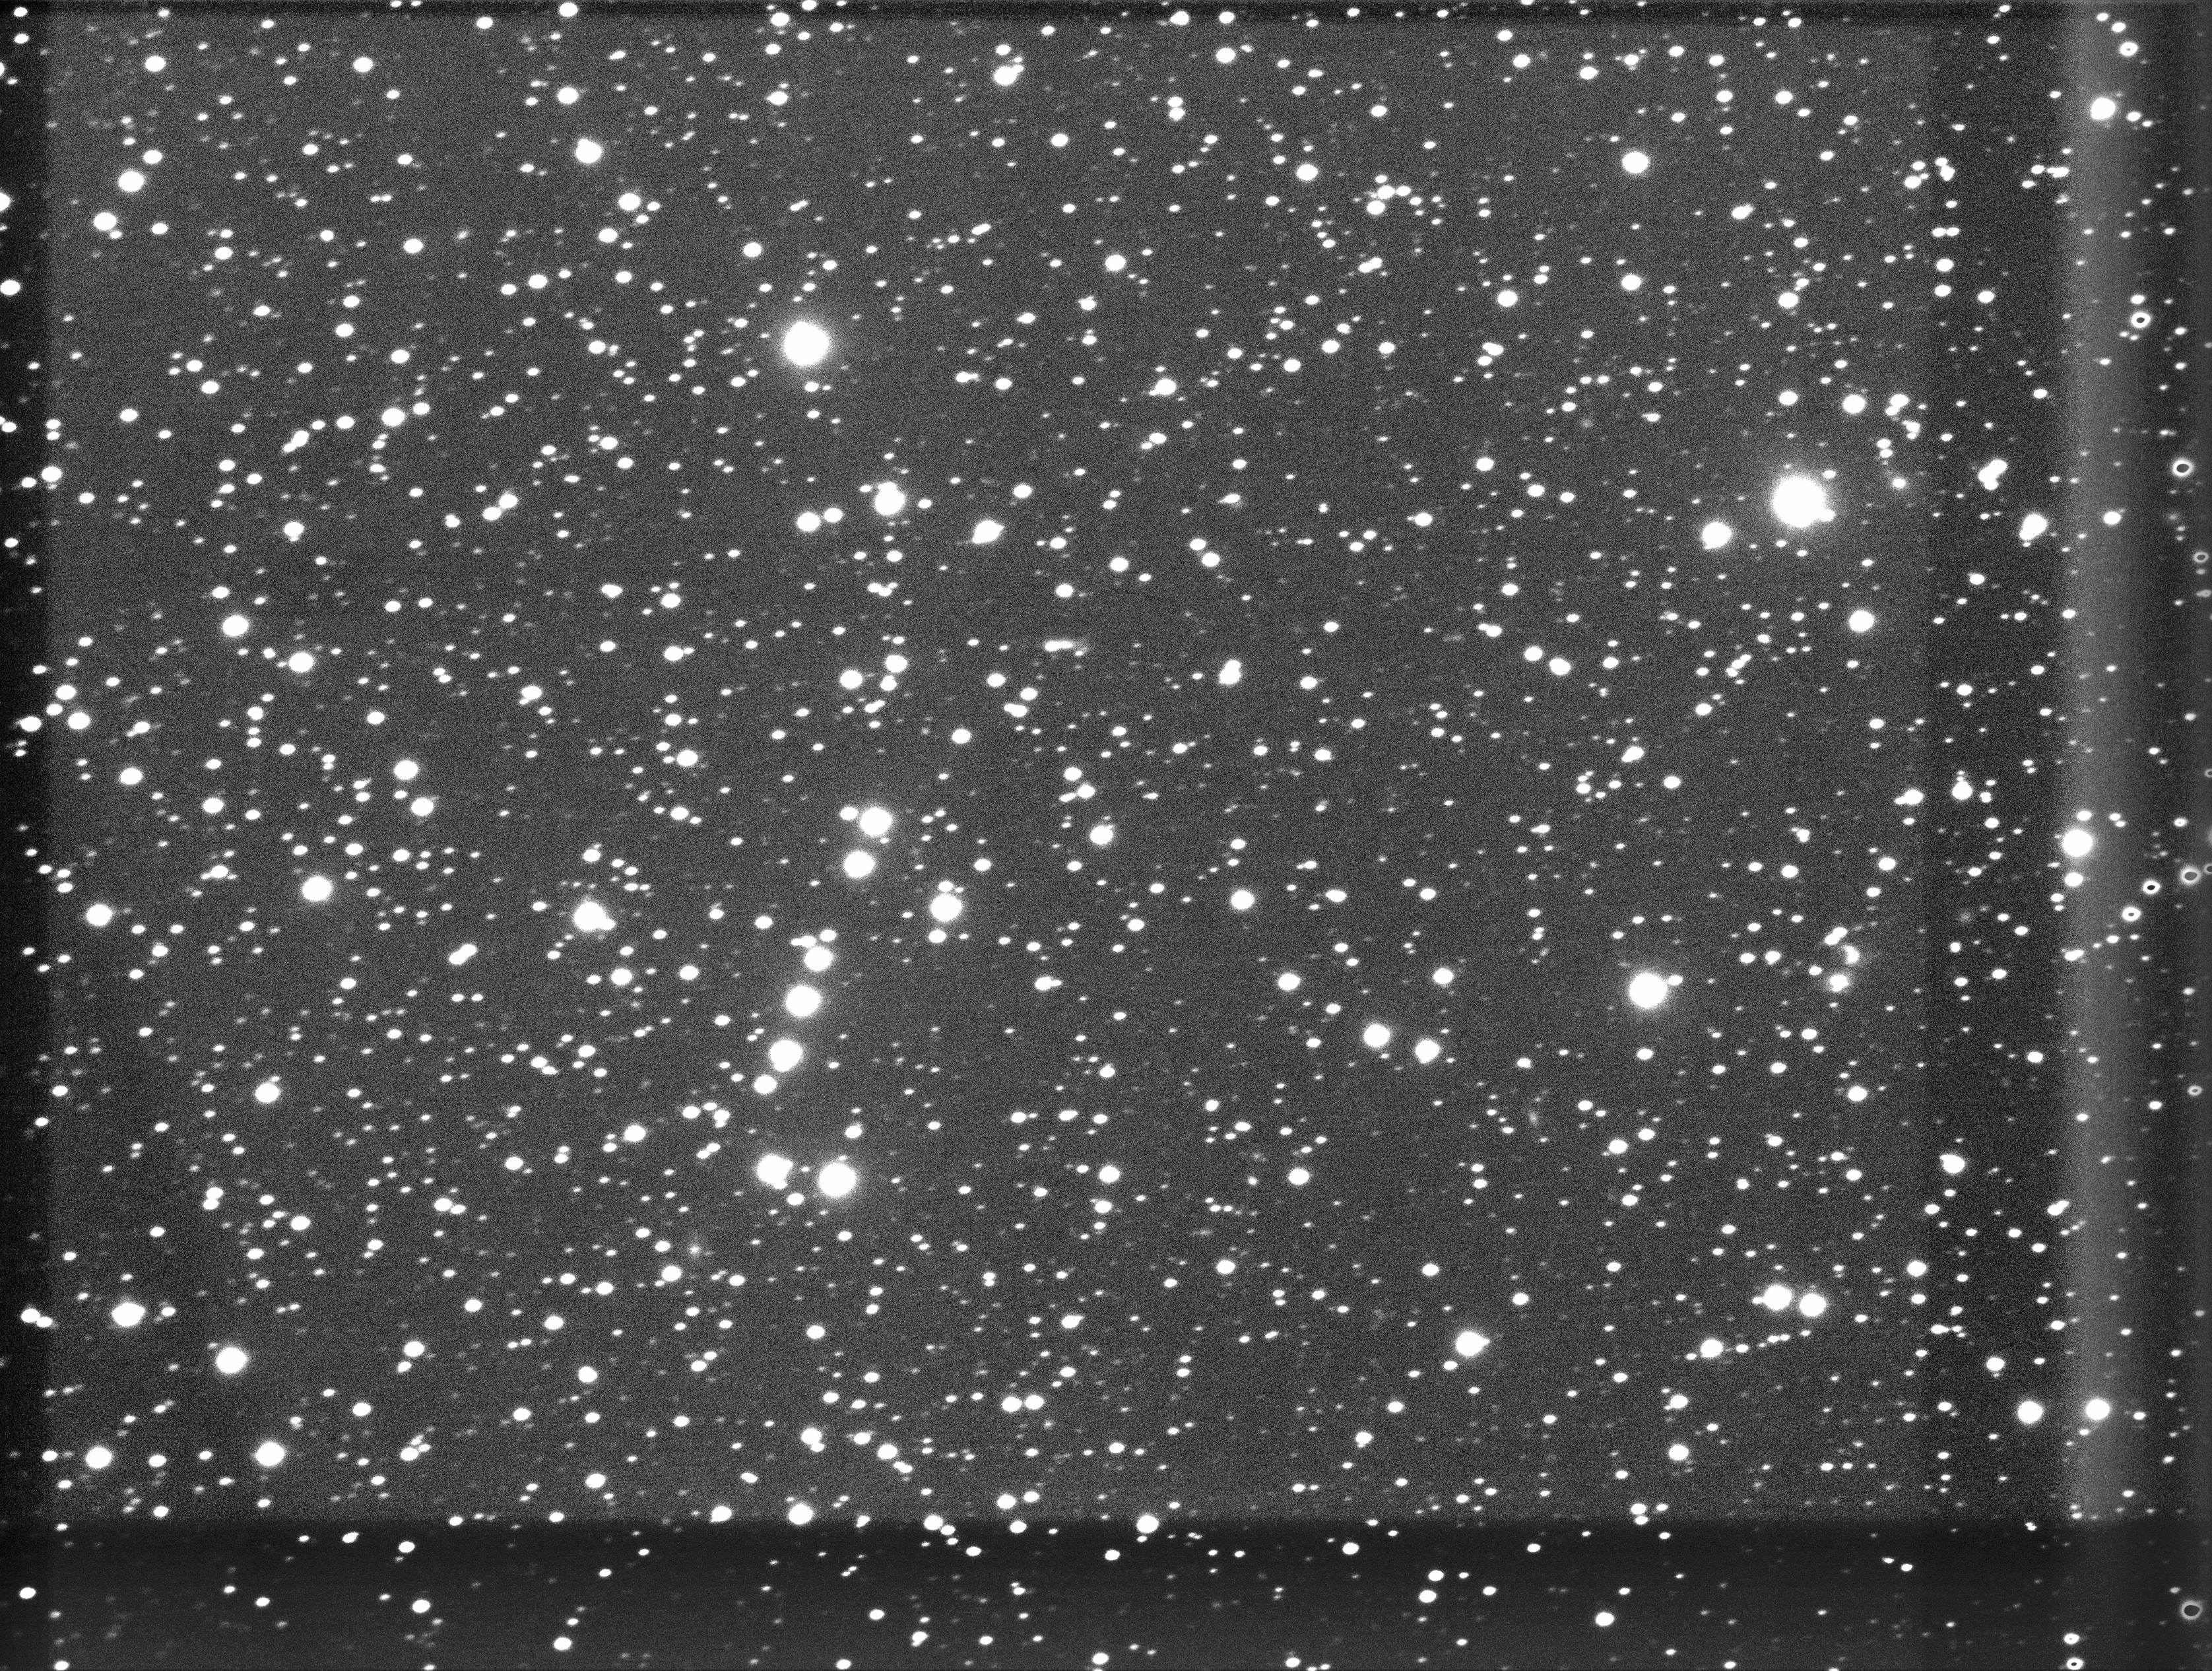
\includegraphics[width=\columnwidth]{figures/deepskynylyr}
    \caption{Deepsky frame of NY Lyr 2017/07/06}
\label{fig:deepskynylyr}
\end{figure}
\begin{figure}[h]
    \centering
    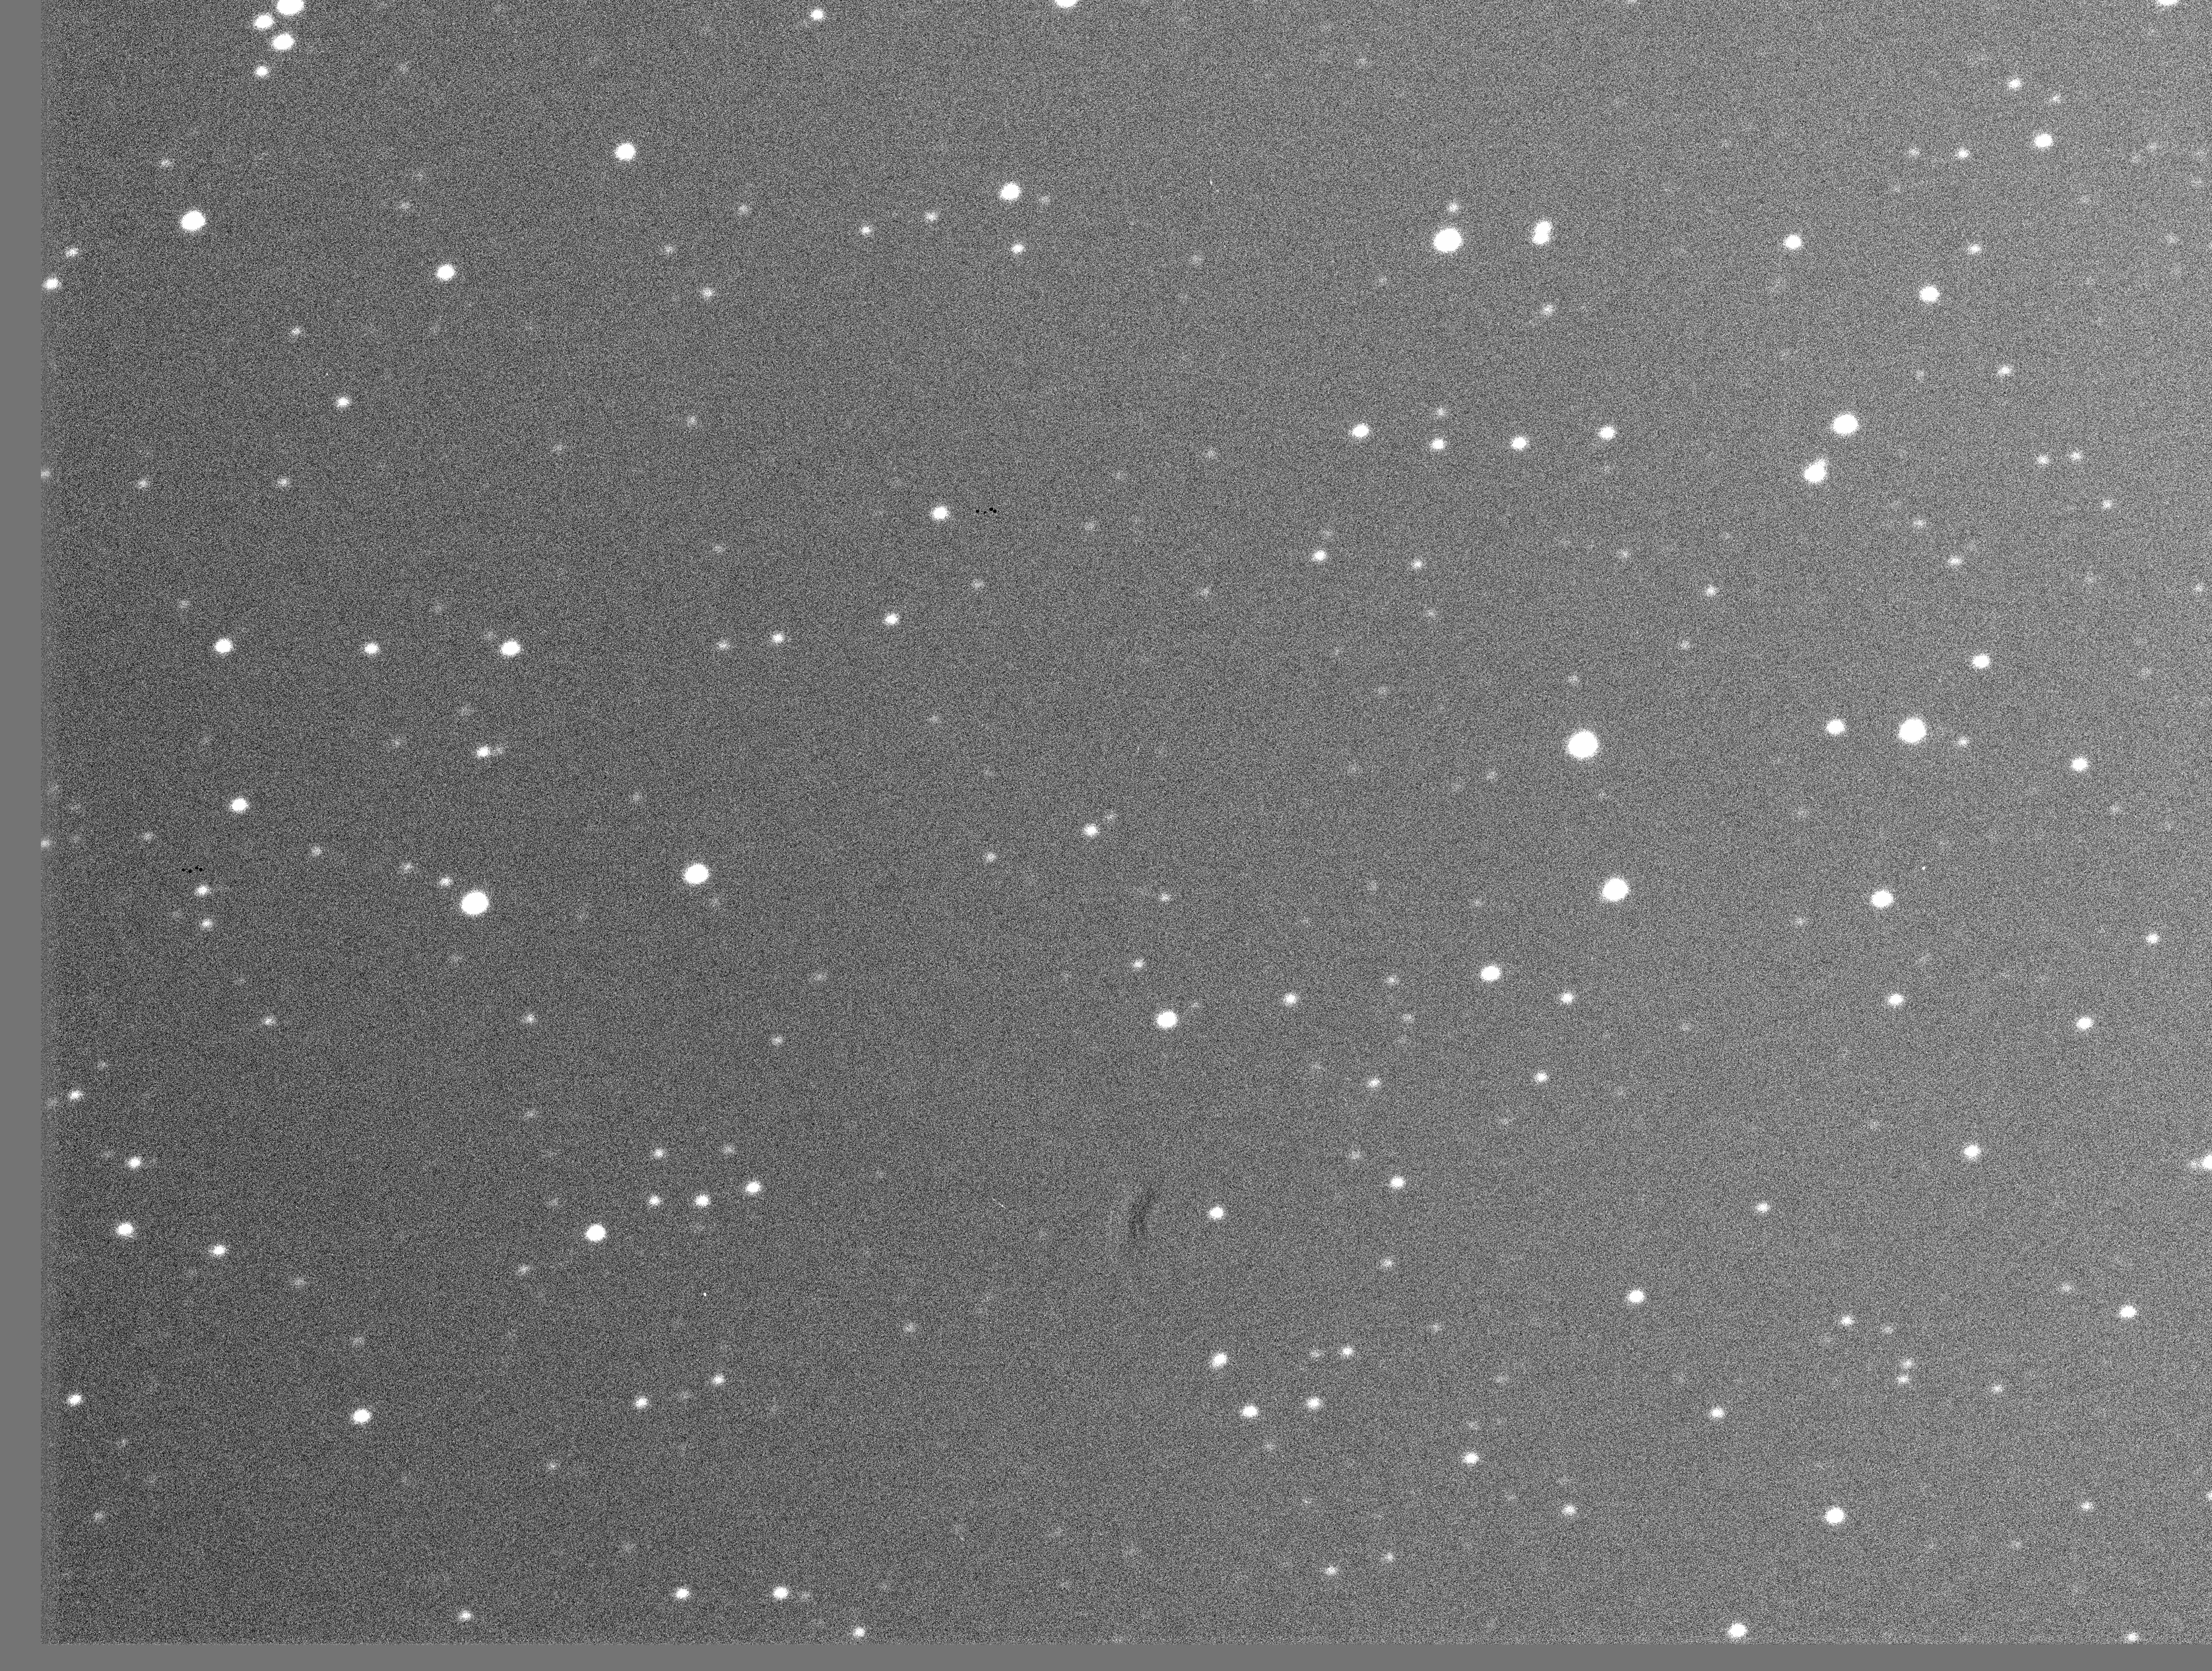
\includegraphics[width=\columnwidth]{figures/deepskyhpaur}
    \caption{Deepsky frame of HP Aur 2017/04/14}
\label{fig:deepskyhpaur}
\end{figure}

\subsection{Known information of targets examined}
Table~\ref{tab:gcvs} are the results given by GCVS Query Form.
\begin{table}[h]
    \centering
    \begin{tabular}{l l l l l l l }
        \toprule
        GCVS & J2000.0 & Type & Max & Min I & Min II & Period \\ \bottomrule
        PR Boo & 151832.01 +445711.6 & EW & 13.44 & 13.85 & 13.79 & 0.3712793 \\ \midrule
        NY Lyr & 191636.86 +342340.5 & EW/KW & 12.7 & 13.2 & 13.1 & 0.44079534 \\ \midrule
        HP Aur & 051021.78 +354746.7 & EA & 11.16  & 11.79 & 11.55 & 1.4228191 \\   
    \bottomrule
    \end{tabular}
    \caption{GCVS entries of observed eclipsing binary}
\label{tab:gcvs}
\end{table}

\subsection{Period analysis by feets}
According to the documentation of feets, the Lomb-Scargle periodogram is
optimized to identify sinusoidal-shaped periodic signals in time-series data. 
Since the targets are all of EW type the expected light curve should be sinusoidal.
Time series data processed by lightcurator is analyzed with feets and the 
extracted feature is called \textit{PeriodLS}, shown in figure~\ref{tab:feets}
\begin{table}
    \centering
    \begin{tabular}{l l c c}
        \toprule
        Object & Date & PeriodLS [$d$] & Period from GCVS [$d$]\\\bottomrule
        PR Boo & 2017/03/30 & 1.200 & 0.3712793 \\ \midrule
               & 2017/04/20 & 0.599 & 0.3712793 \\ \midrule 
        HP Aur & 2017/04/13 & 0.643 & 1.4228191 \\ \midrule 
        NY Lyr & 2017/07/06 & 2.336 & 0.44079534\\
        \bottomrule
    \end{tabular}
    \caption{Period analysis using Lomb-Scargle method as implemented by feets}
\label{tab:feets}
\end{table}

\section{lightcurator Benchmark}
Simple benchmarking was performed on two machines. Results are shown in Table~\ref{tab:benchmark}.
\subsection{Data set}
Data from the observation from 2017/04/20 of PR Boo is used to perform the benchmark.
The data set total size is 3.17 Gigabytes and is 746 frames of 4.1 Megabytes each.
\subsubsection{System specifications}
\begin{description}
    \item[Operating System] macOS Mojave Version 10.14.6
    \item[Processor] 2.9 GHz Intel Core i5
    \item[Memory] 8 GB 1867 MHz DDR3
    \item[Graphics] Intel Iris Graphics 6100 1536 MB
\end{description}

\begin{table}
    \centering
    \begin{tabular}{l c c}
        \toprule
      Process type  & Time to complete deepsky     & Total Processing time\\
      &   [$s$]   &   [$mm:ss$]\\ \bottomrule
      Serial    & 2659.1 & 57:20\\ \midrule
      Parallel  & 1641.2 & 40:26\\
        \bottomrule
    \end{tabular}
    \caption{Comparison of processing types.}
\label{tab:benchmark}
\end{table}

\section{Light curves}
Light curves are generated manually from the time-series catalog generated by lightcurator.

\subsection{PR Boo 2017/03/30}
The raw data from the time-series of PR Boo is shown in figure~\ref{fig:prRAW}.
Magnitudes of comparison stars and their average are plotted and shown along with the variable star in figure~\ref{fig:prCOM}
In figure~\ref{fig:prCHK} one comparison star is picked to compare with the averaged magnitude for comparison to show similarity
in magnitude represented by a flat trend.
The differential photometry light curve result is show in figure~\ref{fig:prPOS}. 

\begin{figure}[h]
    \centering
    \includegraphics{figures/prboo170330RAW.png}
    \caption{Light curve of PR Boo before differential photometry.}
\label{fig:prRAW}
\end{figure}

\begin{figure}[h]
    \centering
    \includegraphics{figures/prboo170330COM.png}
    \caption{Light curve of comparison stars, averaged magnitude for comparison, and PR Boo.}
\label{fig:prCOM}
\end{figure}

\begin{figure}[h]
    \centering
    \includegraphics{figures/prboo170330CHK.png}
    \caption{Difference between comparison star 1 and averaged magnitude for comparison.}
\label{fig:prCHK}
\end{figure}

\begin{figure}[h]
    \centering
    \includegraphics{figures/prboo170330POS.png}
    \caption{Differential photometry of PR Boo.}
\label{fig:prPOS}
\end{figure}

\subsection{PR Boo 2017/04/20}
The raw data from the time-series of PR Boo is shown in figure~\ref{fig:prRAW2}.
Magnitudes of comparison stars and their average are plotted and shown along with the variable star in figure~\ref{fig:prCOM2}
In figure~\ref{fig:prCHK2} one comparison star is picked to compare with the averaged magnitude for comparison to show similarity
in magnitude represented by a flat trend.
The differential photometry light curve result is show in figure~\ref{fig:prPOS2}.
\begin{figure}[h]
    \centering
    \includegraphics{figures/prboo170420RAW.png}
    \caption{Light curve of PR Boo before differential photometry.}
\label{fig:prRAW2}
\end{figure}

\begin{figure}[h]
    \centering
    \includegraphics{figures/prboo170420COM.png}
    \caption{Light curve of comparison stars, averaged magnitude for comparison, and PR Boo.}
\label{fig:prCOM2}
\end{figure}

\begin{figure}[h]
    \centering
    \includegraphics{figures/prboo170420CHK.png}
    \caption{Difference between comparison star 1 and averaged magnitude for comparison.}
\label{fig:prCHK2}
\end{figure}

\begin{figure}[h]
    \centering
    \includegraphics{figures/prboo170420POS.png}
    \caption{Differential photometry of PR Boo.}
\label{fig:prPOS2}
\end{figure}

\subsection{HP Aur 2017/04/13}
The raw data from the time-series of HP Aur is shown in figure~\ref{fig:hpRAW}.
Magnitudes of comparison stars and their average are plotted and shown along with the variable star in figure~\ref{fig:hpCOM}
In figure~\ref{fig:hpCHK} one comparison star is picked to compare with the averaged magnitude for comparison to show similarity
in magnitude represented by a flat trend.
The differential photometry light curve result is show in figure~\ref{fig:hpPOS}.

\begin{figure}[h]
    \centering
    \includegraphics{figures/hpaur170413RAW.png}
    \caption{Light curve of HP Aur before differential photometry.}
\label{fig:hpRAW}
\end{figure}

\begin{figure}[h]
    \centering
    \includegraphics{figures/hpaur170413COM.png}
    \caption{Light curve of comparison stars, averaged magnitude for comparison, and HP Aur.}
\label{fig:hpCOM}
\end{figure}

\begin{figure}[h]
    \centering
    \includegraphics{figures/hpaur170413CHK.png}
    \caption{Difference between comparison star 1 and averaged magnitude for comparison.}
\label{fig:hpCHK}
\end{figure}

\begin{figure}[h]
    \centering
    \includegraphics{figures/hpaur170413POS.png}
    \caption{Differential photometry of HP Aur.}
\label{fig:hpPOS}
\end{figure}

\subsection{NY Lyr 2017/07/06}
The raw data from the time-series of NY Lyr is shown in figure~\ref{fig:nyRAW}.
Magnitudes of comparison stars and their average are plotted and shown along with the variable star in figure~\ref{fig:nyCOM}
In figure~\ref{fig:nyCHK} one comparison star is picked to compare with the averaged magnitude for comparison to show similarity
in magnitude represented by a flat trend.
The differential photometry light curve result is show in figure~\ref{fig:nyPOS}.

\begin{figure}[h]
    \centering
    \includegraphics{figures/nylyr170706RAW.png}
    \caption{Light curve of NY Lyr before differential photometry.}
\label{fig:nyRAW}
\end{figure}

\begin{figure}[h]
    \centering
    \includegraphics{figures/nylyr170706COM.png}
    \caption{Light curve of comparison stars, averaged magnitude for comparison, and NY Lyr.}
\label{fig:nyCOM}
\end{figure}

\begin{figure}[h]
    \centering
    \includegraphics{figures/nylyr170706CHK.png}
    \caption{Difference between comparison star 1 and averaged magnitude for comparison.}
\label{fig:nyCHK}
\end{figure}

\begin{figure}[h]
    \centering
    \includegraphics{figures/nylyr170706POS.png}
    \caption{Differential photometry of NY Lyr.}
\label{fig:nyPOS}
\end{figure}

\section{Eclipsing binary modeling}
Results of the modeling of the eclipsing binary system of PR Boo is shown on figure~\ref{fig:phoebeprboo}.
A comparison of SS Ari and PR Boo parameters are shown on figure~\ref{fig:phoebecompare}.

\begin{figure}[h]
    \centering
    \includegraphics[width=\columnwidth]{figures/phoebecompare.png}
    \caption{Side by side comparison of SS Ari and PR Boo light curve parameters given by PHEOBE.}
\label{fig:phoebecompare}
\end{figure}

\begin{figure}[h]
    \centering
    \includegraphics[width=\columnwidth]{figures/phoebeprboo.png}
    \caption{Model of eclipsing binary system PR Boo generated by PHOEBE.}
\label{fig:phoebeprboo}
\end{figure}
